\twocolumn[{%
\renewcommand\twocolumn[1][]{#1}%
\vspace{-12mm}
\begin{center}
\maketitle
\vspace{-10mm}
\captionsetup{type=figure}
\makebox[\linewidth][c]{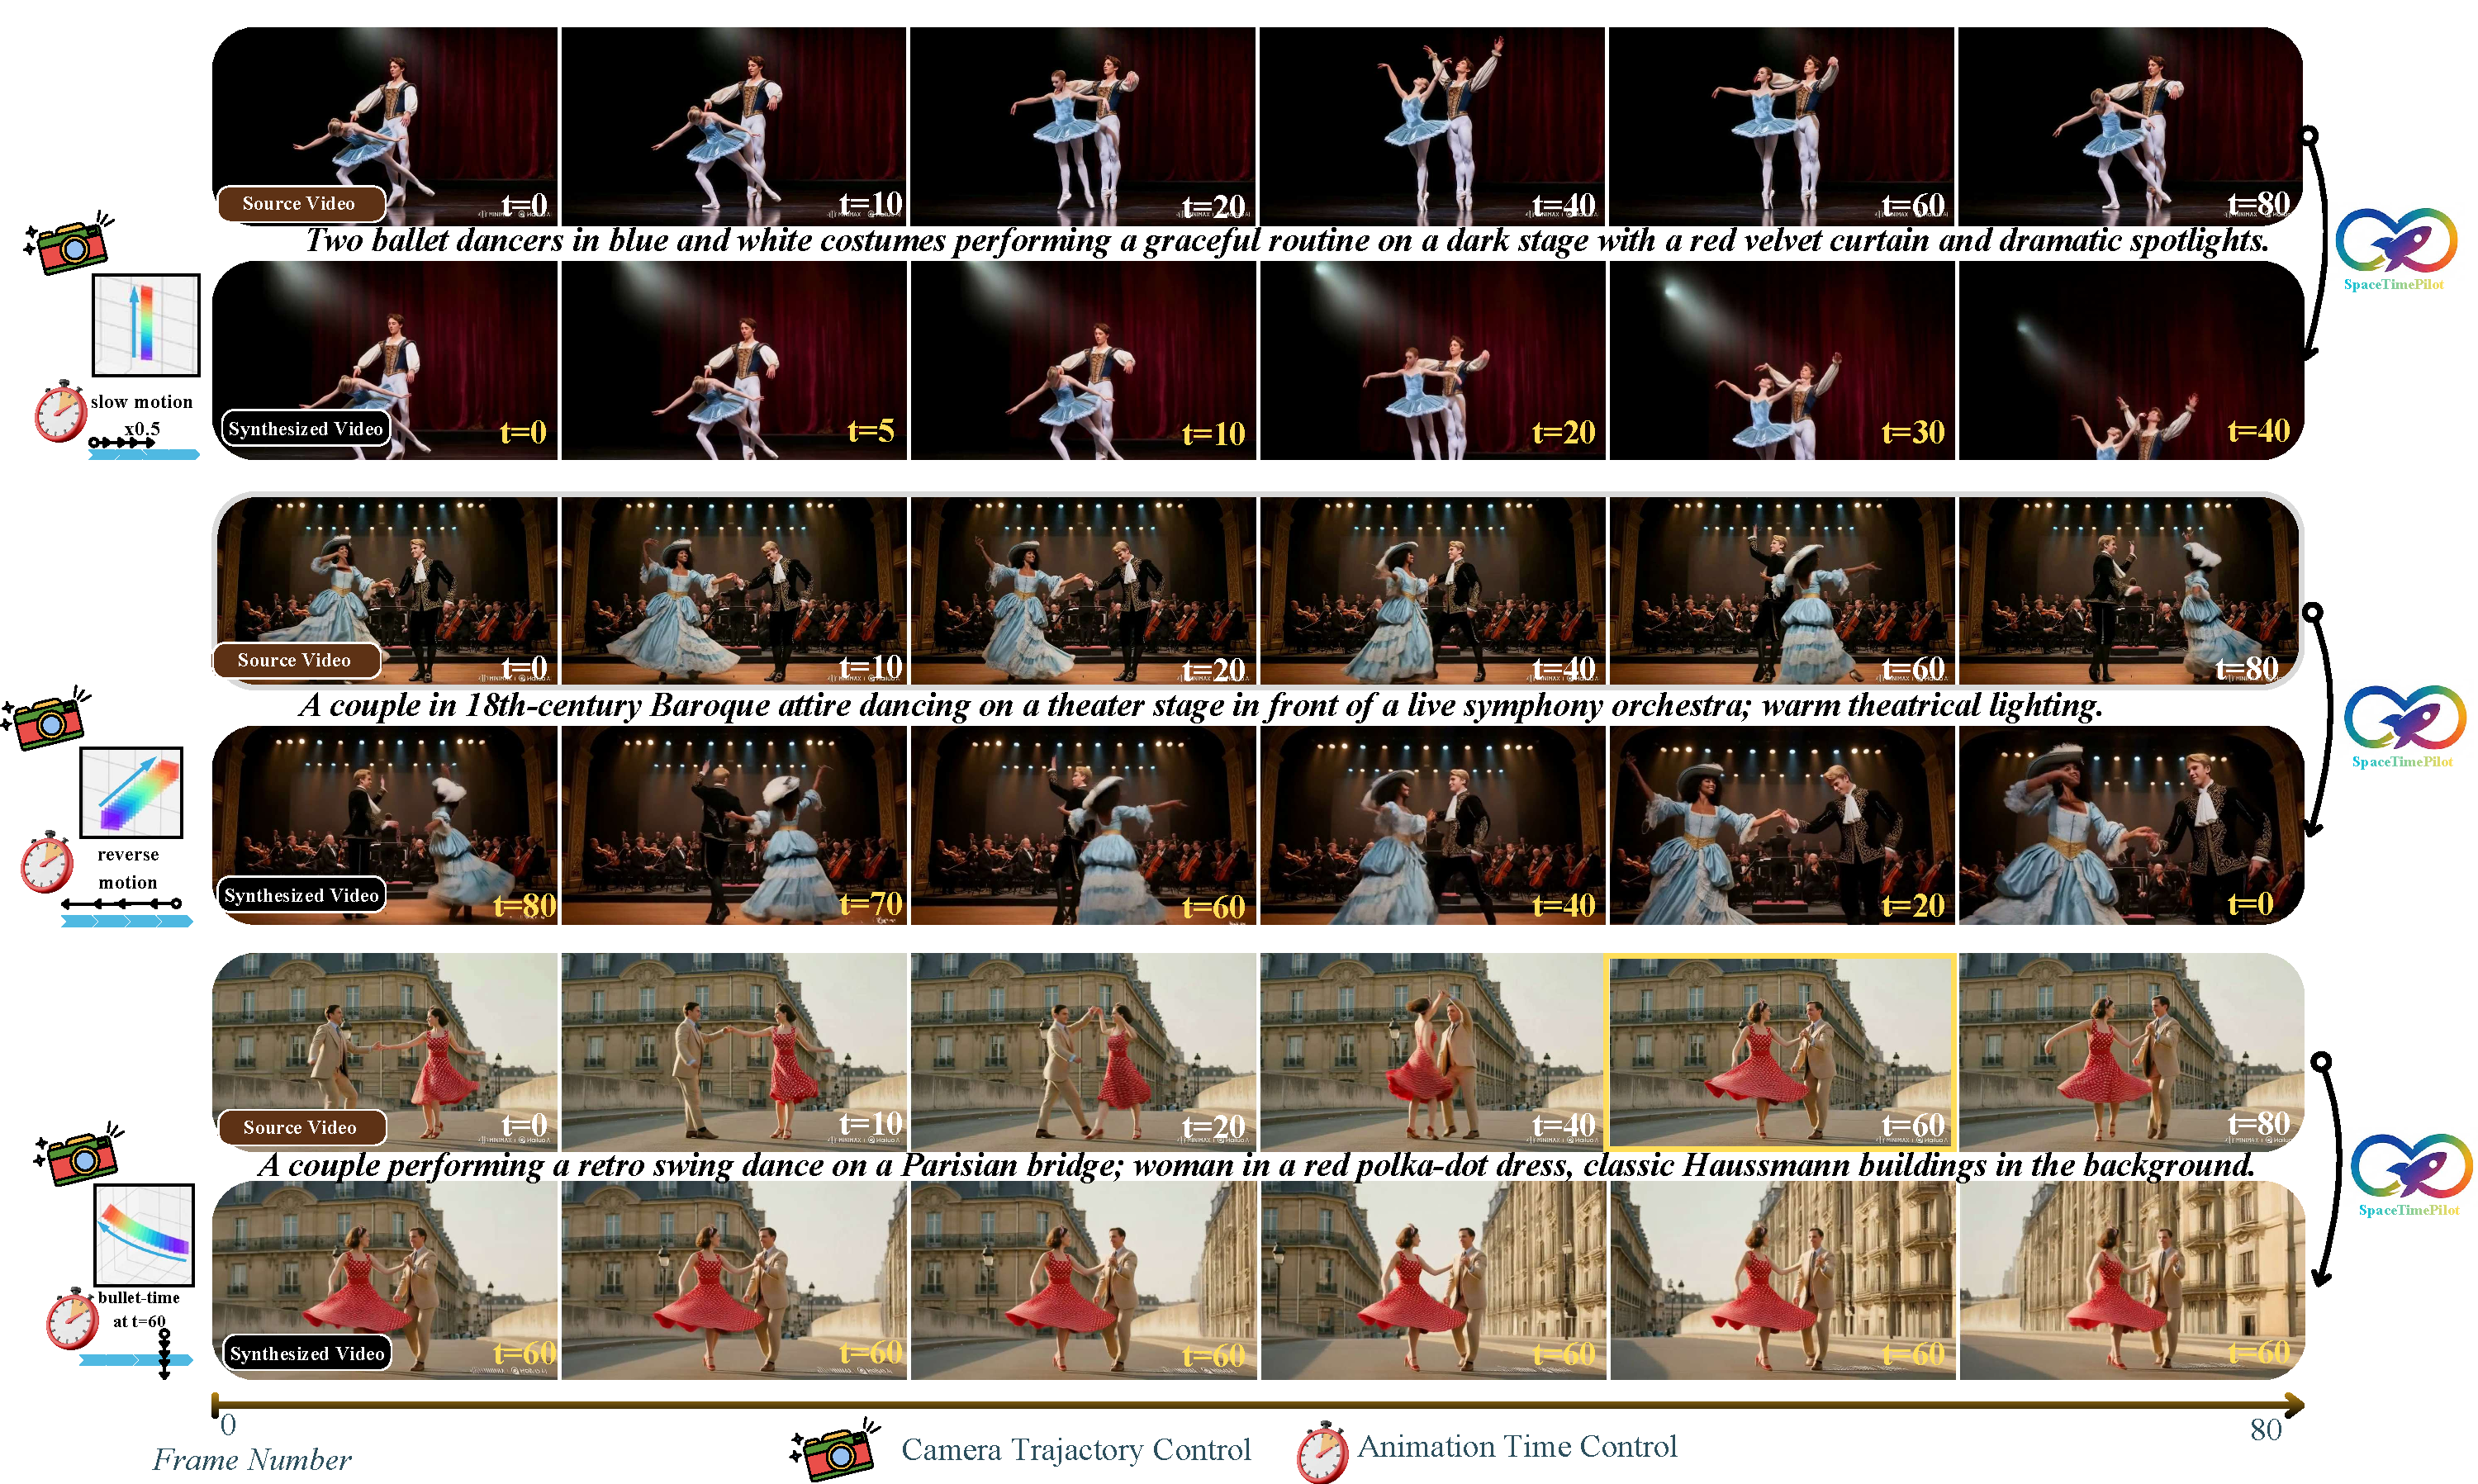
\includegraphics[width=1.1\linewidth]{figures/src_files/teaser_finalfinal.pdf}}
\captionof{figure}{
\textbf{SpaceTimePilot} enables unified control over both camera and time within a single diffusion model, producing continuous and coherent videos along arbitrary space–time trajectories. Given a source video (odd rows), our model synthesizes new videos (even rows) with retimed motion sequences, including slow motion, reverse motion, and bullet time, while precisely controlling camera movement according to a given camera trajectory.
}
\label{fig:teaser}
\end{center}
}]
